% Artigo revisado com base nas observacoes do orientador.
% Dependencias externas: UNESC.cls e referencias.bib.
% Os trechos de codigo foram adaptados da implementacao do projeto.

\documentclass{UNESC}

%==========================================================================
% Pacotes e configuracao
%==========================================================================

\usepackage[T1]{fontenc}
\usepackage[utf8]{inputenc}
\renewcommand{\rmdefault}{phv}
\renewcommand{\sfdefault}{phv}
\usepackage[brazilian]{babel}
\usepackage{graphicx}
\usepackage{hyperref}
\usepackage{quoting}
\usepackage{caption}
\usepackage{enumitem}
\usepackage{float}
\usepackage[hang,flushmargin]{footmisc}
\usepackage{array}
\usepackage{booktabs}
\usepackage{tabularx}
\usepackage{setspace}
\usepackage{listings}
\usepackage{tikz}
\usepackage{placeins}
\usetikzlibrary{arrows.meta,positioning}
\usepackage[alf,recuo=0.0cm,abnt-emphasize=bf]{abntex2cite}

\DeclareCaptionLabelFormat{comtraco}{#1~#2 --}
\captionsetup[figure]{labelformat=comtraco,labelsep=space}
\captionsetup[table]{labelformat=comtraco,labelsep=space}

\hypersetup{
    setpagesize=false,
    colorlinks=true,
    urlcolor=blue,
    linkcolor=black,
    citecolor=black
}

\urlstyle{same}

\newcommand{\codigo}[1]{\texttt{#1}}
\newcommand{\fonteautor}{
    \par\smallskip
    {\footnotesize Fonte: elaboração própria.}
}
\newcolumntype{Y}{>{\raggedright\arraybackslash}X}
\setlength{\emergencystretch}{2em}

\renewcommand{\lstlistingname}{Quadro}
\captionsetup[lstlisting]{labelformat=comtraco,labelsep=space}

\lstdefinestyle{codigotcc}{
    basicstyle=\ttfamily\footnotesize,
    numbers=left,
    numberstyle=\tiny,
    numbersep=8pt,
    frame=single,
    breaklines=true,
    columns=fullflexible,
    keepspaces=true,
    showstringspaces=false,
    captionpos=t,
    tabsize=4,
    aboveskip=0.8em,
    belowskip=0.5em
}

%==========================================================================
% Identificacao
%==========================================================================

\title{ANÁLISE E OTIMIZAÇÃO DE CONSULTAS SQL COM BASE EM LOGS DE EXECUÇÃO EM BANCOS DE DADOS RELACIONAIS}

\author{
Arthur Meira\footnote{
Curso de Ciência da Computação, Universidade do Extremo Sul Catarinense
(Unesc), Criciúma -- Santa Catarina -- Brasil.
arthurmeiraprog@unesc.net
},
Marcel Campos Inocencio\footnote{
Orientador, Curso de Ciência da Computação, Universidade do Extremo Sul
Catarinense (Unesc), Criciúma -- Santa Catarina -- Brasil.
marcel.inocencio@gmail.com
}
}

\begin{document}

\onehalfspacing
\maketitle

%==========================================================================
% Resumo
%==========================================================================

\noindent
\textbf{Resumo:}
Consultas SQL lentas podem gerar gargalos e comprometer o desempenho de sistemas que utilizam bancos de dados relacionais. Este trabalho teve como objetivo desenvolver e avaliar um protótipo para auxiliar na identificação, análise e otimização de consultas SQL no PostgreSQL. A solução utilizou estatísticas agregadas de execução, obtidas por meio da extensão \texttt{pg\_stat\_statements}, e planos de execução para identificar possíveis problemas de desempenho e apresentar recomendações de otimização. Desenvolveu-se uma interface web que permitiu visualizar consultas executadas, consultar métricas, examinar diagnósticos e comparar o desempenho entre versões originais e alternativas. Para avaliar a solução, utilizou-se um banco experimental com dados fictícios de clientes, produtos, pedidos, itens e pagamentos, totalizando 4.648.714 registros. Foram analisadas 12 consultas SQL, cada uma com uma alternativa de otimização, totalizando 240 execuções medidas, sendo 10 repetições por versão de cada consulta. Os resultados demonstraram redução do tempo médio de execução em 10 das 12 consultas avaliadas, com reduções que chegaram a 99,89\%. Entretanto, duas alternativas apresentaram aumento no tempo médio, de até 4,15\%, evidenciando que as modificações propostas nem sempre resultaram em ganhos de desempenho. Concluiu-se que a integração entre estatísticas de execução, análise de planos e validação experimental pode auxiliar na identificação de consultas com possíveis problemas de desempenho e apoiar a avaliação de alternativas de otimização.

\vspace{0.5em}
\noindent
\textbf{Palavras-chave:}
bancos de dados relacionais; consultas SQL; otimização de consultas;
estatísticas de execução; planos de execução.

\vspace{1em}
\noindent
\textbf{ABSTRACT:}
Slow SQL queries can create bottlenecks and impair the performance of systems that use relational databases. This study aimed to develop and evaluate a prototype to support the identification, analysis, and optimization of SQL queries in PostgreSQL. The solution used aggregated execution statistics obtained through the \texttt{pg\_stat\_statements} extension and execution plans to identify potential performance problems and provide optimization recommendations. A web interface was developed to display executed queries, examine metrics, review diagnostic findings, and compare performance between original and alternative query versions. To evaluate the solution, an experimental database containing fictional data on customers, products, orders, order items, and payments was used, totaling 4,648,714 records. Twelve SQL queries were analyzed, each with an optimization alternative, resulting in 240 measured executions, with 10 repetitions per version of each query. The results showed a reduction in mean execution time for 10 of the 12 evaluated queries, with reductions reaching 99.89\%. However, two alternatives showed an increase in mean execution time of up to 4.15\%, demonstrating that the proposed modifications did not always result in performance improvements. It was concluded that integrating execution statistics, execution plan analysis, and experimental validation can assist in identifying queries with potential performance problems and support the evaluation of optimization alternatives.

\noindent
\textbf{Keywords:} relational databases; SQL queries; query optimization; execution statistics; execution plans.

%==========================================================================
% Introducao
%==========================================================================



\section{INTRODUÇÃO}

A linguagem SQL (\textit{Structured Query Language}) é utilizada para consultar e manipular dados em bancos de dados relacionais. O desempenho dessas consultas depende de fatores como volume de registros, filtros, índices e estratégias de execução selecionadas pelo sistema gerenciador de banco de dados (SGBD). Diferentes planos podem produzir os mesmos resultados, mas apresentar custos e tempos de execução distintos \cite{lan2021optimizer}.

A otimização de consultas envolve estimativas de cardinalidade e custo para selecionar estratégias de processamento. Quando essas estimativas são imprecisas, o SGBD pode escolher planos menos eficientes. Características dos dados, como restrições de unicidade e relações entre atributos, também influenciam essas decisões \cite{lan2021optimizer,kossmann2022dependencies}.

Além dos planos de execução, estatísticas como frequência, tempo total e tempo médio permitem identificar consultas que podem comprometer o desempenho das aplicações. A combinação dessas informações com mecanismos de diagnóstico e avaliação de ajustes contribui para orientar decisões de otimização baseadas em evidências \cite{postgresql2026pgstat,huang2023}.

Diante desse contexto, estabeleceu-se a seguinte questão de pesquisa: como integrar estatísticas agregadas de execução e análise de planos para identificar possíveis problemas de desempenho em consultas SQL, propor alternativas de otimização e avaliar experimentalmente seus efeitos no PostgreSQL?

O objetivo geral deste trabalho é desenvolver e avaliar um protótipo para auxiliar na análise e otimização de consultas SQL no PostgreSQL. Como objetivos específicos, buscou-se construir uma base experimental, implementar a coleta de estatísticas, analisar planos de execução, identificar possíveis problemas de desempenho, propor alternativas de otimização e comparar seus resultados e tempos de execução. A solução foi desenvolvida como ferramenta de apoio à decisão, sem aplicar automaticamente as modificações propostas.


%==========================================================================
% Fundamentacao
%==========================================================================

\section{FUNDAMENTAÇÃO TEÓRICA}

\subsection{Otimização e planos de execução}

A otimização de consultas SQL envolve a avaliação de diferentes planos de execução, considerando estimativas de custo e cardinalidade. Essas estimativas auxiliam na escolha das estratégias de processamento, como a ordem das junções e a utilização de índices. Quando imprecisas, podem resultar em planos menos eficientes, reforçando a importância de avaliações experimentais com consultas representativas \cite{lan2021optimizer,leis2025optimizers}.

No PostgreSQL, os planos são organizados em árvores compostas por operações como \codigo{Seq Scan}, \codigo{Index Scan} e \codigo{Hash Join}. O comando \codigo{EXPLAIN} apresenta o plano estimado sem executar a consulta, enquanto \codigo{EXPLAIN ANALYZE} realiza a execução e registra informações como tempo e quantidade de linhas processadas. Como o custo estimado não corresponde diretamente ao tempo em milissegundos, a análise preventiva dos planos e a medição experimental constituem etapas distintas \cite{postgresql2026explain}.

\subsection{Estatísticas e avaliação de desempenho}

A otimização de desempenho em bancos de dados envolve a previsão de desempenho, o diagnóstico de problemas e a realização de ajustes, que representam etapas distintas do processo \cite{huang2023}. No PostgreSQL, a extensão \codigo{pg\_stat\_statements} disponibiliza estatísticas agregadas das consultas executadas, incluindo quantidade de chamadas, tempo total, tempo médio e linhas retornadas ou afetadas. Esses indicadores auxiliam na identificação de consultas que merecem investigação \cite{postgresql2026pgstat}.

Diferentemente dos arquivos de log, que podem registrar execuções individuais, o \codigo{pg\_stat\_statements} reúne informações de múltiplas chamadas. Consultas com estruturas equivalentes podem compartilhar uma mesma entrada estatística, mesmo utilizando diferentes valores nos filtros. Assim, é possível acompanhar seu comportamento acumulado, mas não reconstruir individualmente todas as execuções realizadas \cite{postgresql2026pgstat}.


\subsection{Índices e reescrita de consultas}

Os índices podem melhorar o desempenho de consultas SQL, dependendo da seletividade dos filtros e do volume de dados. Entretanto, leituras sequenciais podem ser mais eficientes quando grande parte da tabela precisa ser acessada \cite{abbasi2024,postgresql2026explain}. A aplicação de funções em filtros também influencia o uso de índices, pois um índice sobre a coluna \codigo{email} não equivale a outro sobre a expressão \codigo{lower(email)}, embora o PostgreSQL permita índices específicos para expressões \cite{postgresql2025expression}.

A reescrita de consultas SQL busca melhorar o desempenho preservando os resultados. Entre as estratégias estão a substituição de filtros por ano por intervalos de datas, a comparação direta de valores normalizados e a reformulação de subconsultas. Contudo, essas alterações devem ser verificadas quanto à correspondência dos resultados e avaliadas experimentalmente, pois não garantem redução no tempo de execução.



\subsection{Validação de alternativas e avaliação experimental de desempenho}

A avaliação de alternativas de otimização de consultas SQL deve considerar a preservação dos resultados e os efeitos das modificações sobre o desempenho. Consultas com estruturas diferentes podem produzir resultados equivalentes, mas apresentar tempos de execução distintos. Por isso, é importante verificar a correspondência dos resultados e medir o desempenho das versões comparadas. No PostgreSQL, o comando \codigo{EXPLAIN ANALYZE} permite obter tempos de execução e informações sobre as operações realizadas, enquanto a opção \codigo{BUFFERS} apresenta dados sobre o acesso aos blocos \cite{kostov2026rewrites,postgresql2026explain}.

A avaliação experimental também deve considerar as características das consultas e as condições de execução. \citeonline{leis2025optimizers} destacam a importância de experimentos representativos na análise dos otimizadores. Nesse contexto, medições repetidas permitem observar variações nos tempos registrados e comparar as alternativas de maneira mais consistente, evitando conclusões baseadas em uma única execução \cite{kostov2026rewrites}.




%==========================================================================
% Materiais e metodos
%==========================================================================


\section{MATERIAIS E MÉTODOS}

\subsection{Etapas do desenvolvimento}


O trabalho foi desenvolvido por meio da construção e avaliação de um protótipo para auxiliar na identificação, análise e otimização de consultas SQL no PostgreSQL. A solução integrou mecanismos de coleta de estatísticas, análise de planos de execução, identificação de possíveis problemas de desempenho e avaliação de alternativas de otimização. Os experimentos foram realizados em ambiente controlado, utilizando um banco de dados com registros fictícios, permitindo analisar o comportamento das consultas e comparar os tempos de execução das versões originais e alternativas.


O desenvolvimento foi organizado em seis etapas: construção do banco experimental, geração e carregamento dos dados, execução de consultas e coleta de estatísticas, análise dos planos de execução, geração de alternativas de otimização e avaliação experimental de desempenho. Na última etapa, verificou-se a correspondência dos resultados entre as consultas originais e suas alternativas, seguida de medições repetidas para comparar os tempos de execução. O Fluxograma 1 apresenta essa sequência.




\begin{center}
\begin{minipage}{\linewidth}
\centering

\textbf{Fluxograma 1 -- Etapas do desenvolvimento}

\vspace{0.3cm}

\begin{tikzpicture}[
    bloco/.style={
        rectangle,
        rounded corners,
        draw=black,
        align=center,
        text width=9.5cm,
        minimum height=0.65cm,
        font=\small
    },
    seta/.style={-{Latex[length=2mm]},thick},
    node distance=0.25cm
]

\node[bloco] (base)
{1. Construção do banco experimental};

\node[bloco,below=of base] (dados)
{2. Geração e carregamento dos dados};

\node[bloco,below=of dados] (coleta)
{3. Execução das consultas e coleta das estatísticas};

\node[bloco,below=of coleta] (analise)
{4. Análise das consultas e dos planos de execução};

\node[bloco,below=of analise] (alternativas)
{5. Geração de alternativas de otimização};

\node[bloco,below=of alternativas] (validacao)
{6. Verificação dos resultados e avaliação experimental};

\draw[seta] (base) -- (dados);
\draw[seta] (dados) -- (coleta);
\draw[seta] (coleta) -- (analise);
\draw[seta] (analise) -- (alternativas);
\draw[seta] (alternativas) -- (validacao);

% Fonte alinhada à borda esquerda do fluxograma
\node[
    anchor=north west,
    inner sep=0pt,
    font=\footnotesize
] at ([yshift=-0.15cm]validacao.south west)
{Fonte: do autor.};

\end{tikzpicture}
\vspace{0.1cm}
\end{minipage}
\end{center}


\subsection{Ambiente de desenvolvimento}

O protótipo foi desenvolvido em Python 3.14.7, utilizando PostgreSQL 18.6 como banco de dados experimental e a biblioteca Psycopg para comunicação com o SGBD. A extensão \codigo{pg\_stat\_statements} foi empregada na coleta de estatísticas de execução, enquanto o SQLite armazenou localmente os dados coletados e os resultados experimentais. As bibliotecas \codigo{pglast} e \codigo{sqlglot} auxiliaram na análise estrutural e na reescrita de consultas SQL. O DBeaver foi utilizado para administração e execução de consultas no banco.

O desenvolvimento ocorreu em dois equipamentos: um computador com processador AMD Ryzen 5 5600X, 32~GB de RAM, SSD Kingston NV2 de 2~TB e Windows 11 Pro; e um notebook com processador Intel Core i5-1135G7, 32~GB de RAM e SSD NVMe de 512~GB. Todas as medições experimentais de desempenho foram realizadas exclusivamente no computador de mesa, utilizando o mesmo ambiente computacional para comparar as versões das consultas.


\subsection{Banco experimental e volumes utilizados}

Criou-se um banco experimental no PostgreSQL composto por cinco tabelas: \codigo{clientes}, \codigo{produtos}, \codigo{pedidos}, \codigo{itens\_pedido} e \codigo{pagamentos}. A estrutura foi organizada de modo que um cliente pudesse realizar diversos pedidos, enquanto cada pedido pudesse conter um ou mais produtos. A tabela \codigo{itens\_pedido} estabeleceu a associação entre pedidos e produtos, e a tabela \codigo{pagamentos} armazenou os registros de pagamento e suas respectivas situações.

Todas as tabelas receberam chaves primárias, e os relacionamentos entre elas foram estabelecidos por meio de chaves estrangeiras. A coluna de e-mail da tabela de clientes recebeu uma restrição de unicidade, que também disponibiliza um índice para operações de busca. Essa estrutura permitiu avaliar consultas com diferentes condições de filtragem e acesso aos dados.

Durante a geração dos dados, cada pedido recebeu dois ou três itens. Essa variação foi utilizada para simular compras com diferentes quantidades de produtos. A quantidade de itens foi escolhida de forma pseudoaleatória, utilizando uma semente fixa para permitir a reprodução dos dados. Além disso, foi gerado um registro de pagamento para cada pedido. Essa quantidade corresponde à regra do gerador, não a uma restrição de unicidade sobre o pedido na tabela de pagamentos.

A Tabela~\ref{tab:base} apresenta a quantidade de registros de cada tabela e sua finalidade na base experimental.

\begin{table}[H]
\centering
\caption{Composição da base experimental}
\label{tab:base}
\small
\begin{tabularx}{\textwidth}{l r Y}
\toprule
\textbf{Tabela} & \textbf{Registros} & \textbf{Finalidade} \\
\midrule
Clientes & 100.000 & Armazenamento dos dados dos clientes, buscas por e-mail e associação aos pedidos. \\
Produtos & 50.000 & Cadastro dos produtos utilizados na composição dos pedidos. \\
Pedidos & 1.000.000 & Registro das compras, consultas por período, junções e agrupamentos. \\
Itens de pedido & 2.498.714 & Associação entre pedidos e produtos, permitindo consultas envolvendo múltiplas tabelas. \\
Pagamentos & 1.000.000 & Registro dos pagamentos associados aos pedidos e suas situações. \\
\midrule
\textbf{Total} & \textbf{4.648.714} & Registros que compõem a base experimental. \\
\bottomrule
\end{tabularx}

\vspace{0.2cm}
{\raggedright\footnotesize Fonte: do autor.\par}
\end{table}


Os volumes de registros foram definidos para avaliar consultas com diferentes características, incluindo buscas por e-mail, filtros por data, junções e agrupamentos. A base foi composta exclusivamente por dados fictícios, permitindo realizar os experimentos em um ambiente controlado.

\subsection{Geração e carregamento dos dados}

A geração dos registros foi realizada por meio do programa \codigo{populate\_database.py}, desenvolvido em Python. Foram configurados 100.000 clientes, 50.000 produtos e 1.000.000 de pedidos, com carregamento em lotes de 10.000 registros. Utilizou-se a semente 2026 para controlar as escolhas pseudoaleatórias, permitindo reproduzir a geração dos dados quando mantidos o código e os parâmetros utilizados.


O Quadro~\ref{cod:geracao} apresenta parte da lógica utilizada na geração dos pedidos, ilustrando como os registros foram produzidos para compor a base experimental.



\begin{lstlisting}[
    style=codigotcc,
    language=Python,
    caption={Recorte da geração dos pedidos},
    label={cod:geracao}
]
rng = random.Random(args.seed)

customer_id = popular_id(
    rng, customer_count, 0.20, 0.80
)

year = rng.choices(
    (2024, 2025, 2026),
    weights=(20, 30, 50),
    k=1
)[0]

status = rng.choices(
    ("pendente", "pago", "enviado", "entregue", "cancelado"),
    weights=(12, 13, 20, 48, 7),
    k=1
)[0]
\end{lstlisting}
\noindent{\footnotesize Fonte: do autor.\par}


A geração dos dados utilizou distribuições pseudoaleatórias para simular diferentes frequências de compras. Entre os clientes, 80\% das escolhas foram direcionadas aos primeiros 20\% dos identificadores, enquanto 70\% das seleções de produtos foram direcionadas aos primeiros 10\% do catálogo. Os pedidos foram distribuídos entre 2024, 2025 e 2026, com probabilidades de 20\%, 30\% e 50\%, respectivamente, considerando apenas os meses de janeiro a agosto para 2026.

Os valores dos pedidos foram calculados a partir dos preços e das quantidades dos produtos, utilizando centavos inteiros e conversão para \codigo{Decimal}. Os pagamentos receberam situações relacionadas às dos pedidos, e os e-mails foram gerados em letras minúsculas, característica relevante para os testes de otimização. O carregamento utilizou o comando \codigo{COPY}, por meio da biblioteca Psycopg e do método \codigo{write\_row}, em lotes de até 10.000 pedidos com seus itens e pagamentos \cite{postgresql2025populate,psycopgcopy}.

\begin{lstlisting}[
    style=codigotcc,
    language=Python,
    caption={Carregamento de pedidos, itens e pagamentos em lotes},
    label={cod:carga}
]
for first_id in range(1, args.pedidos + 1, args.lote):
    stop_id = min(
        first_id + args.lote,
        args.pedidos + 1
    )

    orders, items, payments = make_order_batch(
        first_id,
        stop_id,
        counts["itens_pedido"] + 1,
        args.clientes,
        prices,
        rng
    )

    copy_rows(cursor, "pedidos", orders)
    copy_rows(cursor, "itens_pedido", items)
    copy_rows(cursor, "pagamentos", payments)

    counts["itens_pedido"] += len(items)
\end{lstlisting}
\noindent{\footnotesize Fonte: do autor.\par}

Antes do carregamento, o programa verificou o nome do banco de dados e se as tabelas estavam vazias. Caso fossem encontrados registros existentes, o processo era interrompido para evitar alterações nos dados já armazenados. A transação foi confirmada após a conclusão do carregamento.

Após a inserção dos registros, executou-se o comando \codigo{ANALYZE} nas cinco tabelas para atualizar as estatísticas utilizadas pelo planejador de consultas do PostgreSQL \cite{postgresql2025populate}. A conferência dos dados foi realizada por meio de consultas organizadas no arquivo \codigo{sql/validate\_population.sql}, que verificaram as quantidades de registros e informações como valores, datas e situações dos pedidos e pagamentos.

\subsection{Consultas e avaliação experimental}

Foram selecionadas 12 consultas SQL, identificadas de C01 a C12, envolvendo diferentes operações, como filtros, junções, agrupamentos, ordenações e subconsultas. Para cada consulta original, foi definida uma alternativa de otimização, permitindo comparar o desempenho entre as duas versões.

A avaliação foi realizada no banco experimental desenvolvido para o trabalho. Inicialmente, verificou-se se as consultas originais e suas alternativas produziam resultados correspondentes nas condições do experimento. Em seguida, realizou-se uma execução de aquecimento por versão e 10 medições de cada consulta original e alternativa, em ordem embaralhada. Os tempos foram obtidos por meio do comando \codigo{EXPLAIN ANALYZE} do PostgreSQL, totalizando 240 execuções medidas. Esse total não inclui as execuções de aquecimento e as verificações adicionais dos resultados.

A Tabela~\ref{tab:carga} apresenta as consultas utilizadas na avaliação experimental e a quantidade de execuções medidas em cada caso.

\begin{table}[H]
\centering
\caption{Consultas utilizadas na avaliação experimental}
\label{tab:carga}

\begin{minipage}{\textwidth}
\small
\begin{tabularx}{\linewidth}{c Y c}
\toprule
\textbf{Consulta} & \textbf{Operação principal} & \textbf{Execuções medidas} \\
\midrule
C01 & Consulta de pedidos por ano. & 20 \\
C02 & Busca de clientes por e-mail. & 20 \\
C03 & Contagem de pedidos por cliente. & 20 \\
C04 & Ranking anual de compras. & 20 \\
C05 & Cálculo dos totais mensais de vendas. & 20 \\
C06 & Consulta de pedidos anuais com clientes. & 20 \\
C07 & Cálculo do total anual de pedidos. & 20 \\
C08 & Cálculo do valor anual dos pedidos. & 20 \\
C09 & Consulta de pedidos por ano e situação. & 20 \\
C10 & Consulta de pedidos anuais por cliente. & 20 \\
C11 & Consulta de pedidos anuais por maior valor. & 20 \\
C12 & Contagem de pedidos por cliente e cidade. & 20 \\
\midrule
\textbf{Total} & \textbf{12 consultas e 12 alternativas} & \textbf{240} \\
\bottomrule
\end{tabularx}

\vspace{0.2cm}
{\raggedright\footnotesize Fonte: do autor.\par}
\end{minipage}
\end{table}

Antes das medições de desempenho, verificou-se o funcionamento das consultas e a correspondência dos resultados entre as versões originais e suas alternativas. A verificação considerou a quantidade de registros, as colunas retornadas e a comparação dos resultados obtidos na base experimental.

As medições foram realizadas em ordem embaralhada, com o objetivo de reduzir a influência da sequência de execução sobre os resultados. Os tempos foram obtidos diretamente pelo PostgreSQL, utilizando \codigo{EXPLAIN ANALYZE} com informações de acesso aos blocos de dados. Os testes foram realizados em um único computador, sem a simulação de usuários concorrentes.

\subsection{Coleta das estatísticas e medição dos tempos}

A coleta de estatísticas utilizou a extensão \codigo{pg\_stat\_statements} do PostgreSQL, que disponibiliza informações agregadas sobre as consultas executadas, como quantidade de chamadas, tempo total, tempo médio e linhas retornadas. Por meio da opção \codigo{Atualizar consultas}, o protótipo consulta essas informações e as armazena localmente em SQLite, permitindo acompanhar o histórico das coletas e identificar consultas que merecem investigação \cite{postgresql2026pgstat}.

A avaliação de desempenho utilizou o comando \codigo{EXPLAIN ANALYZE}, com as opções \codigo{BUFFERS} e \codigo{TIMING FALSE}, para medir os tempos de execução e obter informações sobre o acesso aos blocos de dados \cite{postgresql2026explain}. Foram realizadas 10 medições por versão para cada uma das 12 consultas avaliadas, com os resultados armazenados pelo protótipo e utilizados para calcular médias e medianas. Os tempos correspondem às medições do PostgreSQL com a instrumentação do \codigo{EXPLAIN ANALYZE}, sem incluir a transferência completa dos resultados ao cliente.

\subsection{Análise preventiva dos planos}

A análise preventiva utilizou o comando \codigo{EXPLAIN} em formato JSON, com a opção \codigo{ANALYZE FALSE}, permitindo examinar planos estimados sem executar as consultas. O protótipo analisa operações como leituras de tabelas, filtros, junções e ordenações, além das estimativas de linhas. Para consultas com parâmetros sem valores definidos, podem ser utilizados planos genéricos \cite{postgresql2026explain}. Quando existem estatísticas históricas correspondentes e valores definidos para a consulta, o analisador também pode comparar as linhas estimadas com a média histórica por execução, obtida pelo \codigo{pg\_stat\_statements} \cite{postgresql2026pgstat}.

A identificação de possíveis problemas ocorre por meio de regras que avaliam características das consultas e dos planos. Cada sinal identificado recebe uma pontuação, cuja soma é limitada a 10 pontos, classificando a consulta em níveis de atenção baixo, médio ou alto. A Tabela~\ref{tab:regras} apresenta os critérios e as respectivas pontuações utilizados pelo analisador.


\begin{table}[H]
\centering
\caption{Critérios utilizados pelo analisador}
\label{tab:regras}

\begin{minipage}{\textwidth}
\footnotesize
\begin{tabularx}{\linewidth}{Y Y c}
\toprule
\textbf{Sinal} & \textbf{Condição observada} & \textbf{Pontos} \\
\midrule
Seleção ampla & Utilização de \codigo{SELECT *}. & 1 \\
Varredura sequencial filtrada & Leitura sequencial com filtro em tabela com pelo menos 50.000 linhas estimadas. & 3 \\
Função no filtro & Utilização de funções como \codigo{LOWER} e \codigo{EXTRACT} em filtros. & 2 \\
Ordenação extensa & Ordenação de pelo menos 10.000 linhas estimadas. & 2 \\
Laço aninhado & Produto das estimativas dos filhos de pelo menos 1.000.000. & 2 \\
Resultado volumoso & Estimativa de pelo menos 100.000 linhas de saída. & 3 \\
Divergência de linhas & Diferença de pelo menos dez vezes entre as linhas estimadas e a média histórica, quando a comparação é possível. & 3 \\
Subplano & Presença de subplano identificado no plano de execução. & 2 \\
\bottomrule
\end{tabularx}

\vspace{0.2cm}
{\raggedright\footnotesize Fonte: do autor.\par}
\end{minipage}
\end{table}

A soma dos pontos foi limitada a 10. Pontuações de zero a dois foram classificadas como atenção baixa; de três a seis, média; e de sete a dez, alta. Essa classificação foi definida para organizar os possíveis problemas identificados pelo analisador, não representando uma medida estatística de criticidade nem uma previsão do tempo de execução.

Os sinais identificados foram acompanhados de informações que justificam os alertas e, quando aplicável, de recomendações de otimização. Por exemplo, uma leitura sequencial com filtro pode indicar a necessidade de avaliar o uso de índices, enquanto uma função aplicada a uma coluna filtrada pode indicar possibilidades de reescrita da consulta. As recomendações servem como apoio à análise, sem realizar alterações automáticas nas consultas ou na estrutura do banco de dados.



\subsection{Comparação e validação das alternativas}

O protótipo apresenta alternativas de otimização para determinados padrões de consultas SQL, incluindo a substituição de filtros por ano por intervalos de datas, a remoção de funções em condições específicas e a reformulação de subconsultas. Antes das medições, o sistema verifica a correspondência entre os resultados das versões original e alternativa, considerando as colunas retornadas, a quantidade de registros e as assinaturas dos resultados. Caso sejam identificadas diferenças, a comparação de desempenho é interrompida.

A avaliação experimental contemplou 12 consultas SQL, identificadas de C01 a C12, cada uma com uma alternativa de otimização. Para cada par, realizou-se uma execução de aquecimento por versão, seguida de 10 medições de cada consulta, em ordem embaralhada, totalizando 240 execuções medidas. Esse total não inclui as etapas de aquecimento e verificação dos resultados.

Os tempos foram obtidos por meio do comando \codigo{EXPLAIN ANALYZE}, com as opções \codigo{BUFFERS} e \codigo{TIMING FALSE}, e utilizados para calcular médias e medianas. Os resultados foram armazenados pelo protótipo, permitindo consultar o histórico das avaliações e identificar os casos em que as alternativas apresentaram melhoria ou piora no desempenho.



\subsection{Interface e verificação funcional}

O protótipo foi desenvolvido com uma interface web local, utilizando HTML, CSS e JavaScript, integrada a um servidor Python responsável pela comunicação com os módulos de coleta, análise e avaliação de consultas SQL.

A interface permite visualizar consultas executadas no PostgreSQL, atualizar suas estatísticas por meio da opção \codigo{Atualizar consultas} e examinar indicadores como quantidade de chamadas e tempos de execução. Também possibilita analisar planos estimados, consultar os problemas identificados, visualizar alternativas de otimização e comparar seus desempenhos. Os resultados das avaliações são armazenados em um histórico para consulta posterior.

A verificação funcional foi realizada por meio de testes automatizados, abrangendo a coleta de estatísticas, a análise das consultas, a geração de recomendações e a comparação dos resultados. Em uma execução documentada, 58 testes foram concluídos com sucesso, contribuindo para verificar o funcionamento das principais funcionalidades implementadas.


%==========================================================================
% Resultados
%==========================================================================

\section{RESULTADOS E DISCUSSÃO}

\subsection{Resultados da avaliação experimental}

A avaliação experimental contemplou 12 consultas SQL, identificadas de C01 a C12, cada uma com uma alternativa de otimização. Foram realizadas 240 execuções medidas, sendo 10 repetições da versão original e 10 da alternativa para cada consulta. A verificação dos resultados foi concluída com sucesso nos 12 casos avaliados, considerando os dados e parâmetros utilizados nos experimentos.

As alternativas apresentaram redução do tempo médio de execução em 10 das 12 consultas. O maior ganho foi observado na busca por e-mail (C02), com redução de aproximadamente 99,89\%. Por outro lado, as consultas C04 e C06 apresentaram aumento do tempo médio de 4,15\% e 3,13\%, respectivamente. Esses resultados demonstram que as modificações propostas podem melhorar o desempenho, mas seus efeitos dependem das características de cada consulta.

A Tabela~\ref{tab:ranking} apresenta os tempos médios obtidos nas 12 consultas avaliadas, comparando as versões originais e suas alternativas de otimização. A variação percentual indica a redução ou o aumento do tempo médio de execução, calculado a partir dos valores completos antes do arredondamento.

\begin{table}[H]
\centering
\caption{Comparação dos tempos médios de execução}
\label{tab:ranking}

\begin{minipage}{\textwidth}
\small
\begin{tabular*}{\linewidth}{@{\extracolsep{\fill}}c r r r@{}}
\toprule
\textbf{Consulta} & \textbf{Original (ms)} & \textbf{Alternativa (ms)} & \textbf{Variação} \\
\midrule
C01 & 92,88 & 64,22 & -30,86\% \\
C02 & 22,25 & 0,0235 & -99,89\% \\
C03 & 377,81 & 139,83 & -62,99\% \\
C04 & 241,52 & 251,56 & +4,15\% \\
C05 & 179,68 & 165,34 & -7,98\% \\
C06 & 118,32 & 122,02 & +3,13\% \\
C07 & 93,25 & 64,08 & -31,28\% \\
C08 & 79,74 & 58,94 & -26,08\% \\
C09 & 113,40 & 70,36 & -37,96\% \\
C10 & 126,90 & 99,68 & -21,44\% \\
C11 & 98,42 & 82,17 & -16,52\% \\
C12 & 1.196,96 & 140,22 & -88,29\% \\
\bottomrule
\end{tabular*}

\vspace{0.2cm}
{\raggedright\footnotesize Fonte: do autor.\par}
\end{minipage}
\end{table}

Os resultados demonstraram redução do tempo médio em 10 das 12 consultas avaliadas. O maior ganho percentual ocorreu na C02, referente à busca por e-mail, com redução de aproximadamente 99,89\%. A C12 também apresentou uma redução expressiva, passando de 1.196,96 para 140,22 milissegundos.

Por outro lado, as consultas C04 e C06 apresentaram aumento do tempo médio, de aproximadamente 4,15\% e 3,13\%, respectivamente. Esses resultados mostram que a reescrita de uma consulta não garante melhoria de desempenho, reforçando a importância de avaliar experimentalmente as alternativas propostas.



\subsection{Demonstração do funcionamento do protótipo}

Para demonstrar o funcionamento do protótipo, utilizou-se a consulta C03, referente à contagem de pedidos por cliente. A Figura~\ref{fig:consultas_observadas} apresenta a interface de consultas observadas, com estatísticas coletadas do PostgreSQL. Após a seleção de uma consulta, o sistema permite examinar sua instrução SQL, conforme a Figura~\ref{fig:consulta_investigada}, e visualizar as evidências identificadas na análise preventiva, apresentadas na Figura~\ref{fig:evidencias_plano}. Nessa análise, o PostgreSQL gerou um plano genérico, sem os valores originais dos parâmetros. Para gerar a alternativa apresentada na Figura~\ref{fig:sugestao_otimizacao}, foram informados os valores 1 e 10 para o intervalo de clientes, correspondentes ao caso C03 avaliado.

\begin{figure}[!htbp]
\centering
\caption{Interface de consultas observadas}
\label{fig:consultas_observadas}
\begin{minipage}{0.95\textwidth}
\centering
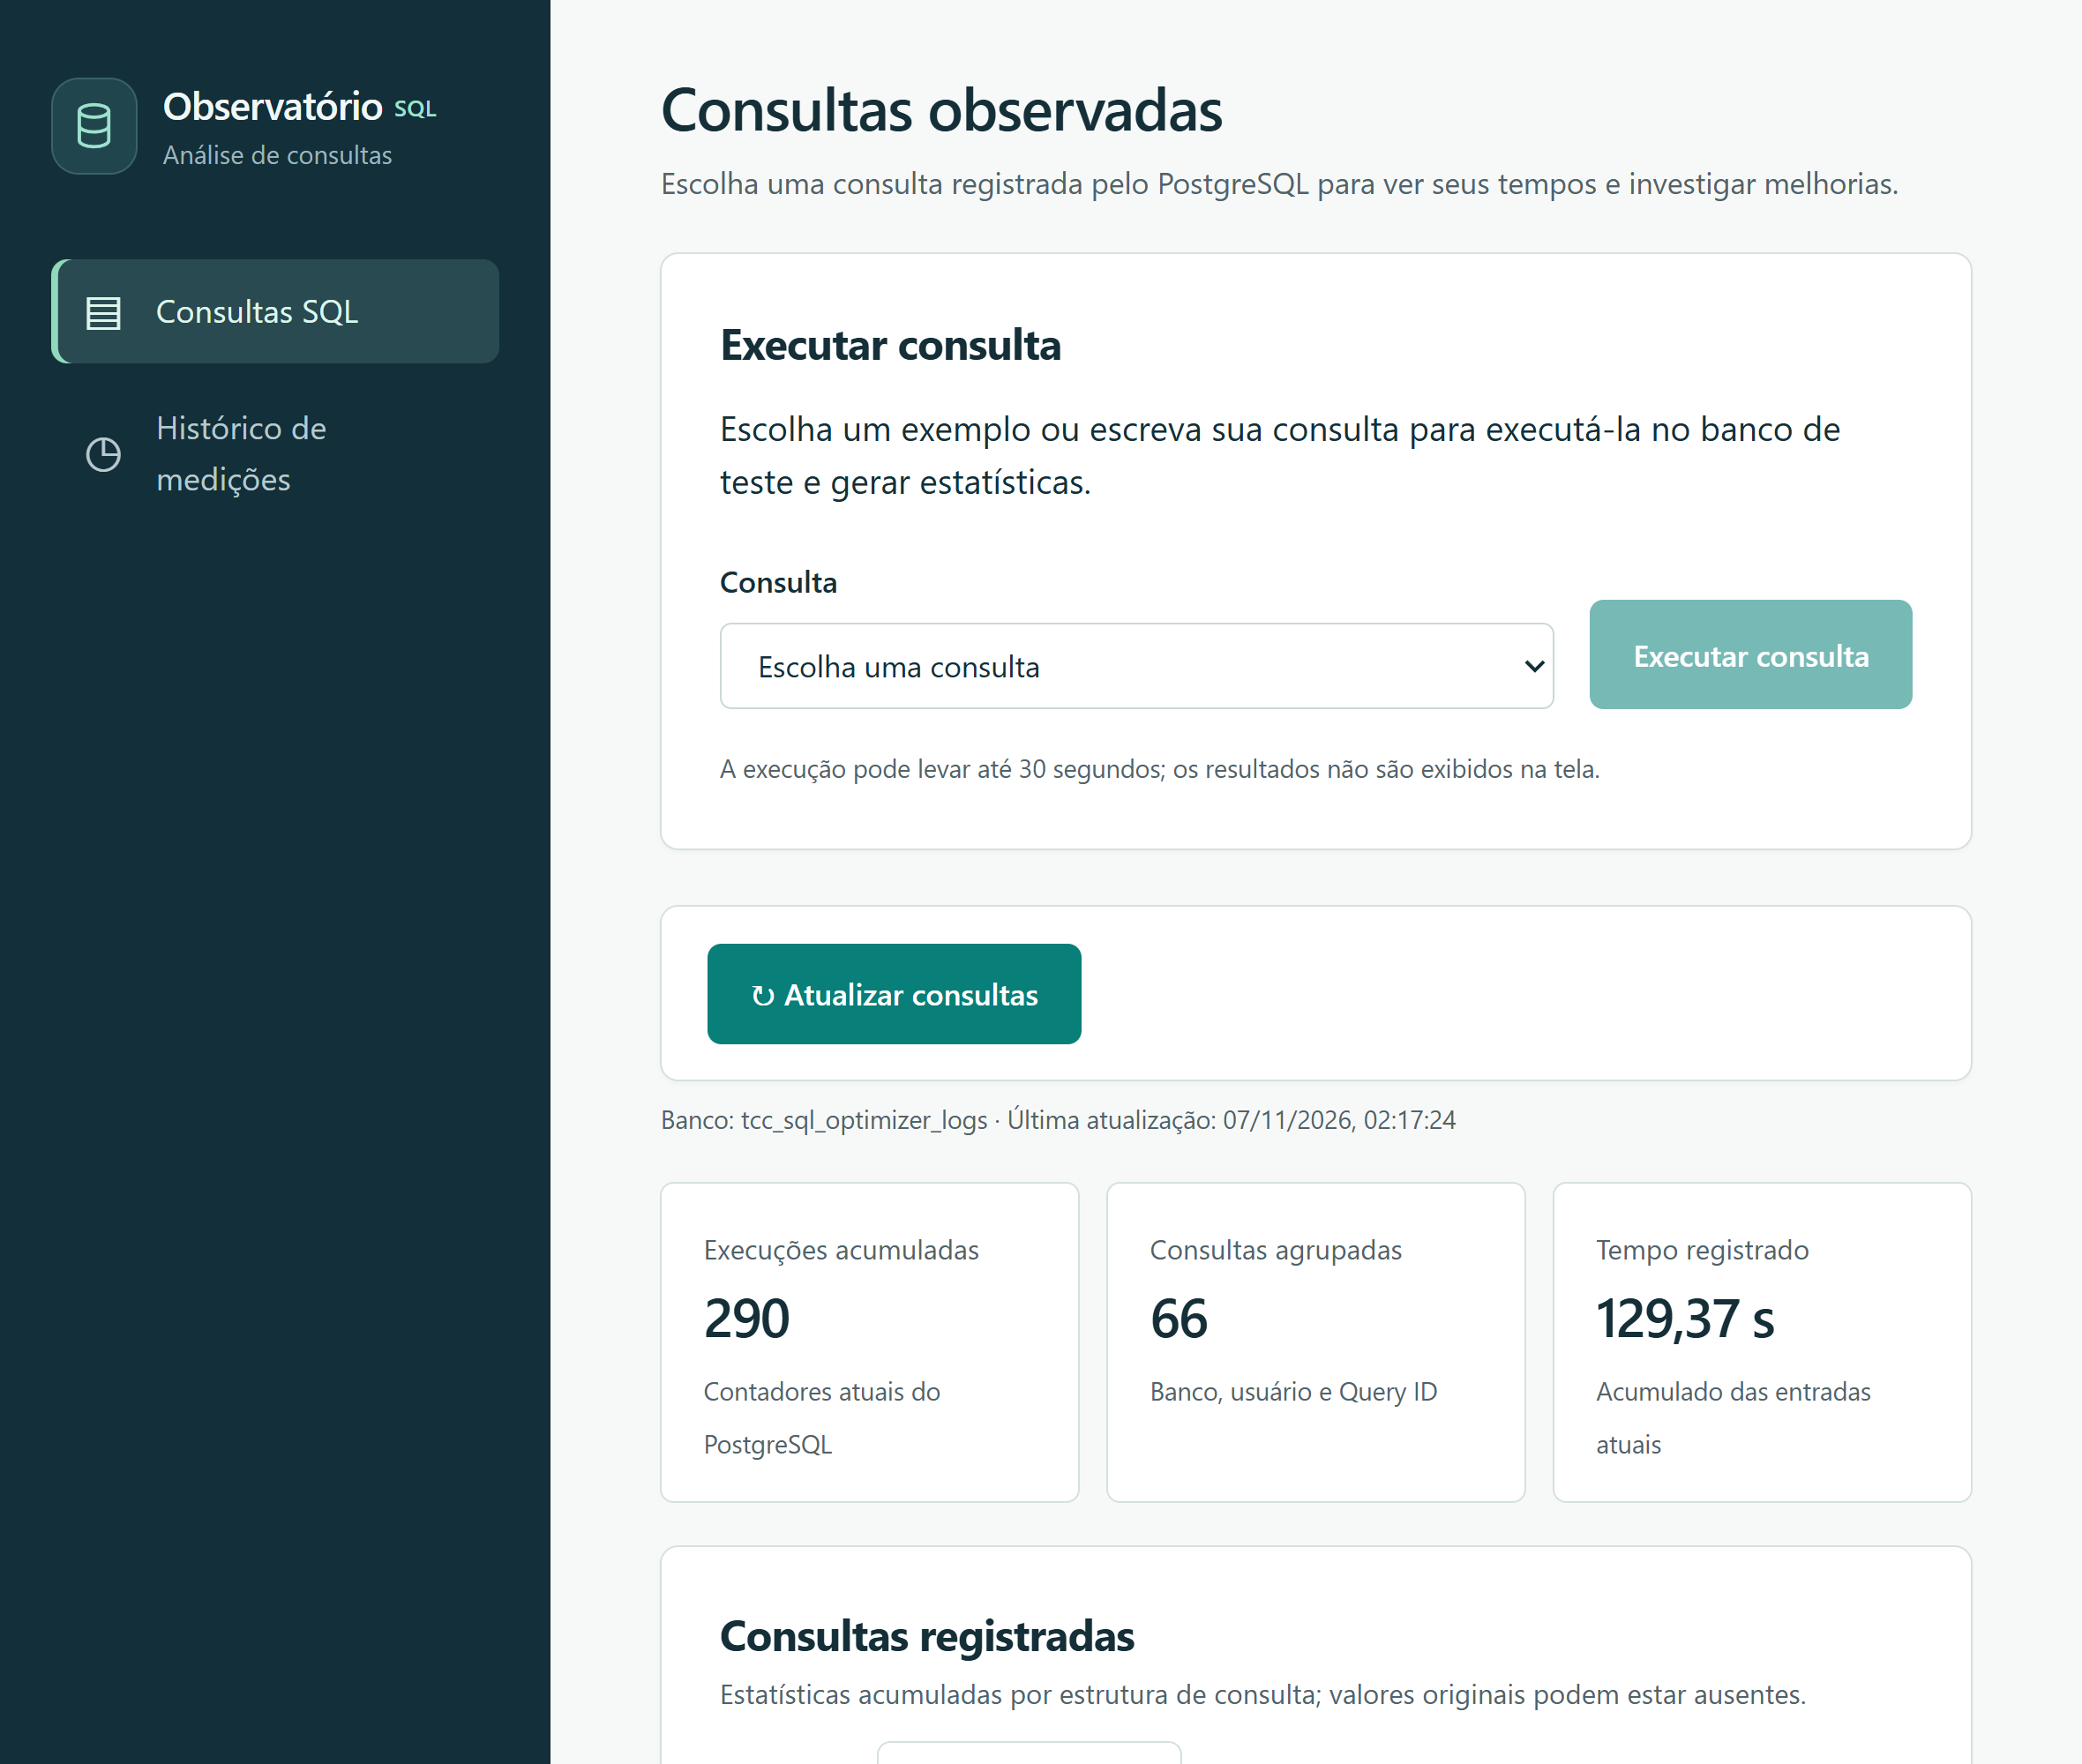
\includegraphics[width=\linewidth]{Figs/01_consultas_observadas.png}
\par\smallskip
{\raggedright\footnotesize Fonte: do autor.\par}
\end{minipage}
\end{figure}

\begin{figure}[!htbp]
\centering
\caption{Consulta selecionada para análise}
\label{fig:consulta_investigada}
\begin{minipage}{0.95\textwidth}
\centering
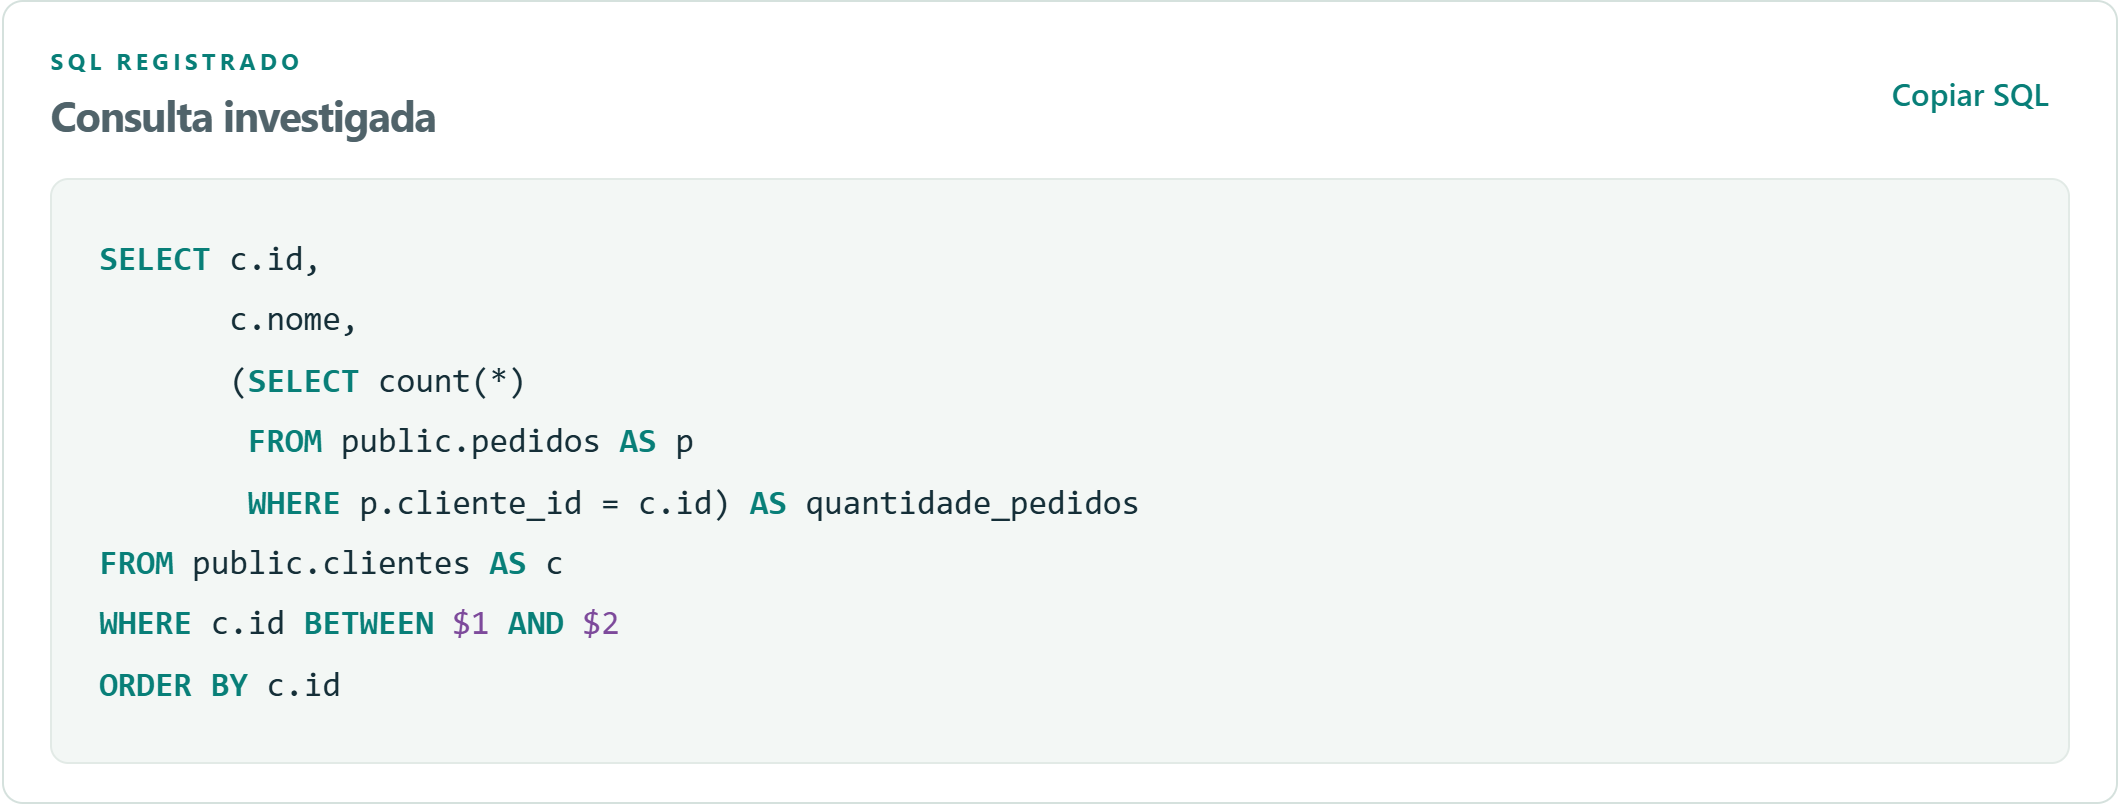
\includegraphics[width=\linewidth]{Figs/02_consulta_investigada.png}
\par\smallskip
{\raggedright\footnotesize Fonte: do autor.\par}
\end{minipage}
\end{figure}

\begin{figure}[!htbp]
\centering
\caption{Evidências identificadas na consulta C03}
\label{fig:evidencias_plano}
\begin{minipage}{0.95\textwidth}
\centering
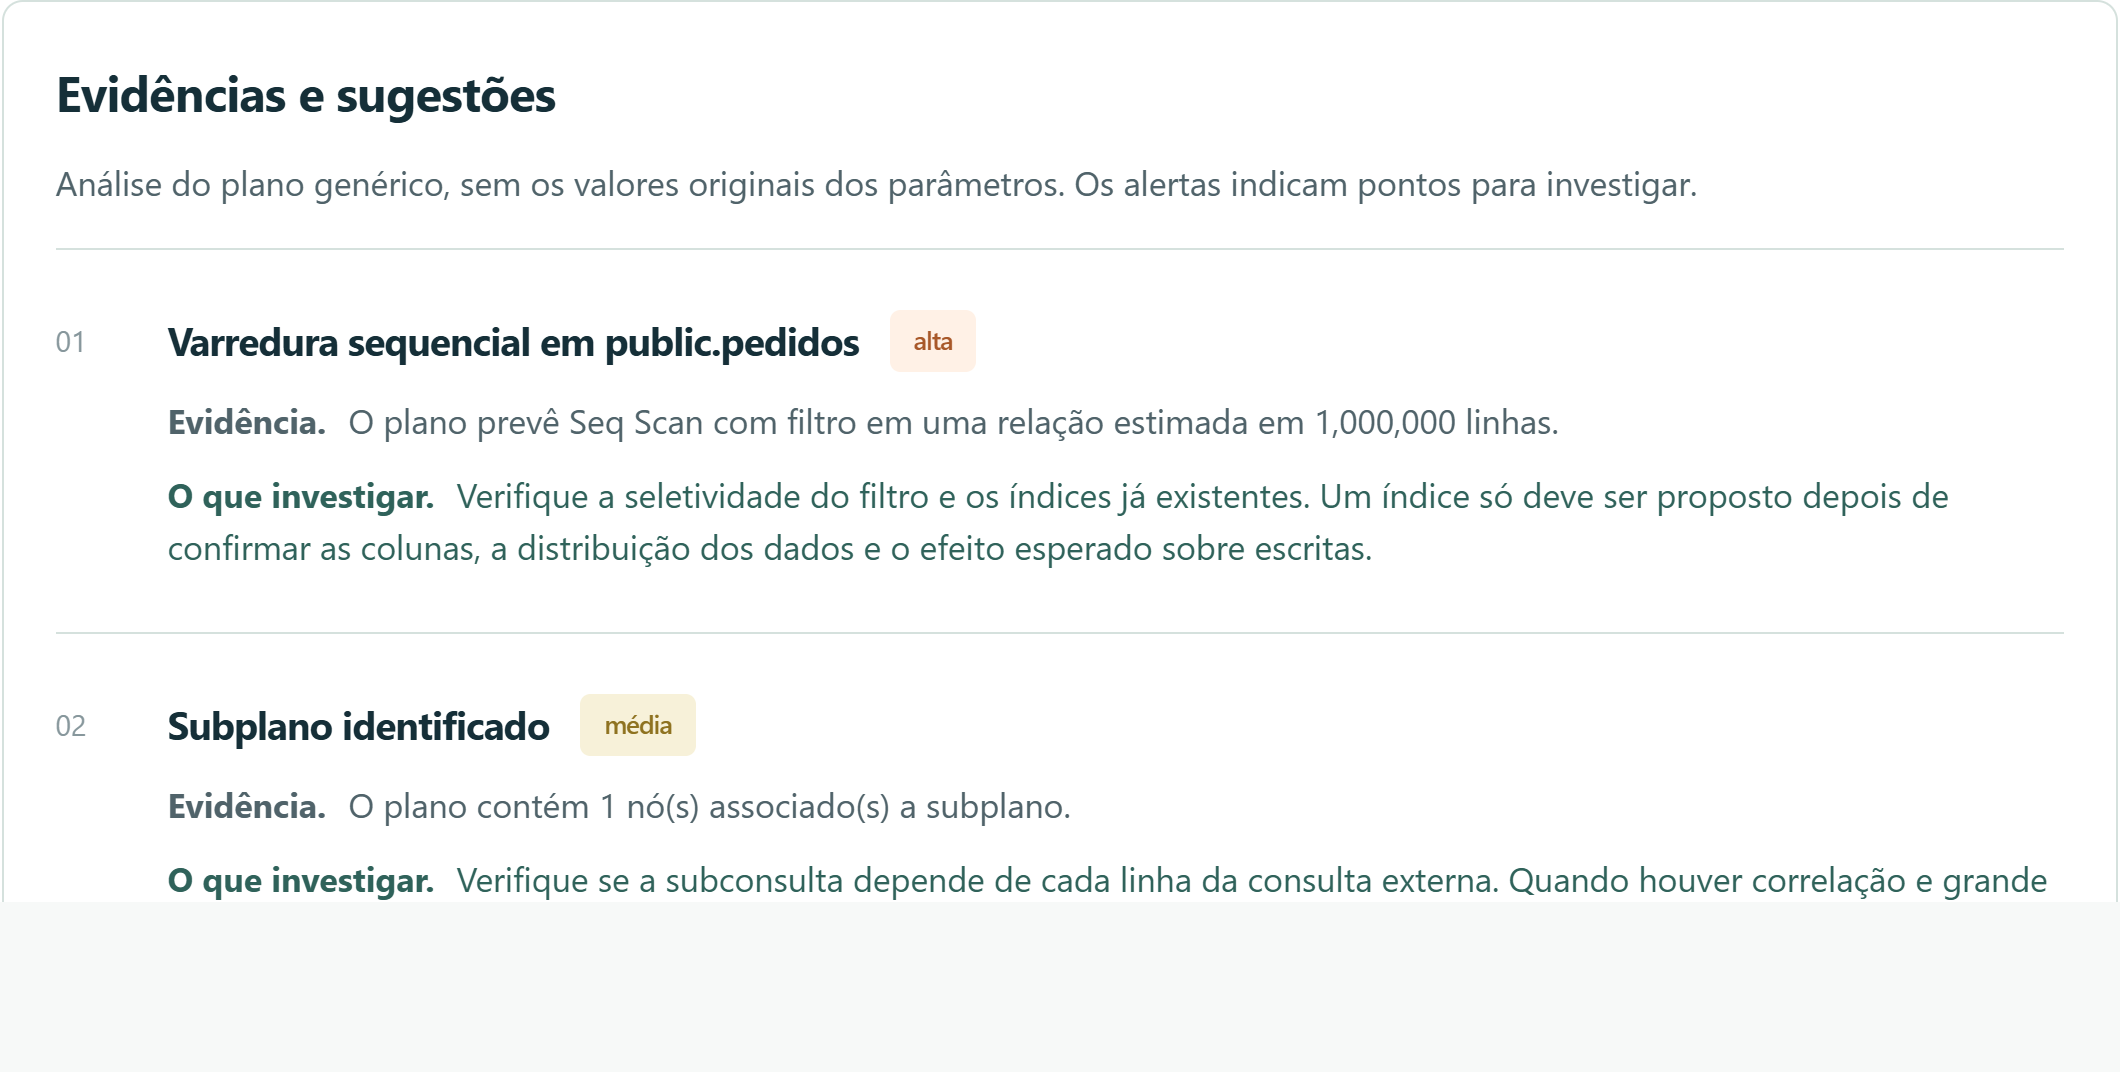
\includegraphics[width=\linewidth]{Figs/03_evidencias_plano.png}
\par\smallskip
{\raggedright\footnotesize Fonte: do autor.\par}
\end{minipage}
\end{figure}

A partir da análise, o protótipo apresenta uma alternativa de otimização, ilustrada na Figura~\ref{fig:sugestao_otimizacao}. Nessa captura, a indicação de que a consulta ainda não foi medida refere-se à análise aberta para a demonstração. Os custos estimados apresentados pelo planejador não representam, isoladamente, uma redução comprovada no tempo de execução.

\begin{figure}[!htbp]
\centering
\caption{Alternativa de otimização apresentada para a C03}
\label{fig:sugestao_otimizacao}
\begin{minipage}{0.95\textwidth}
\centering
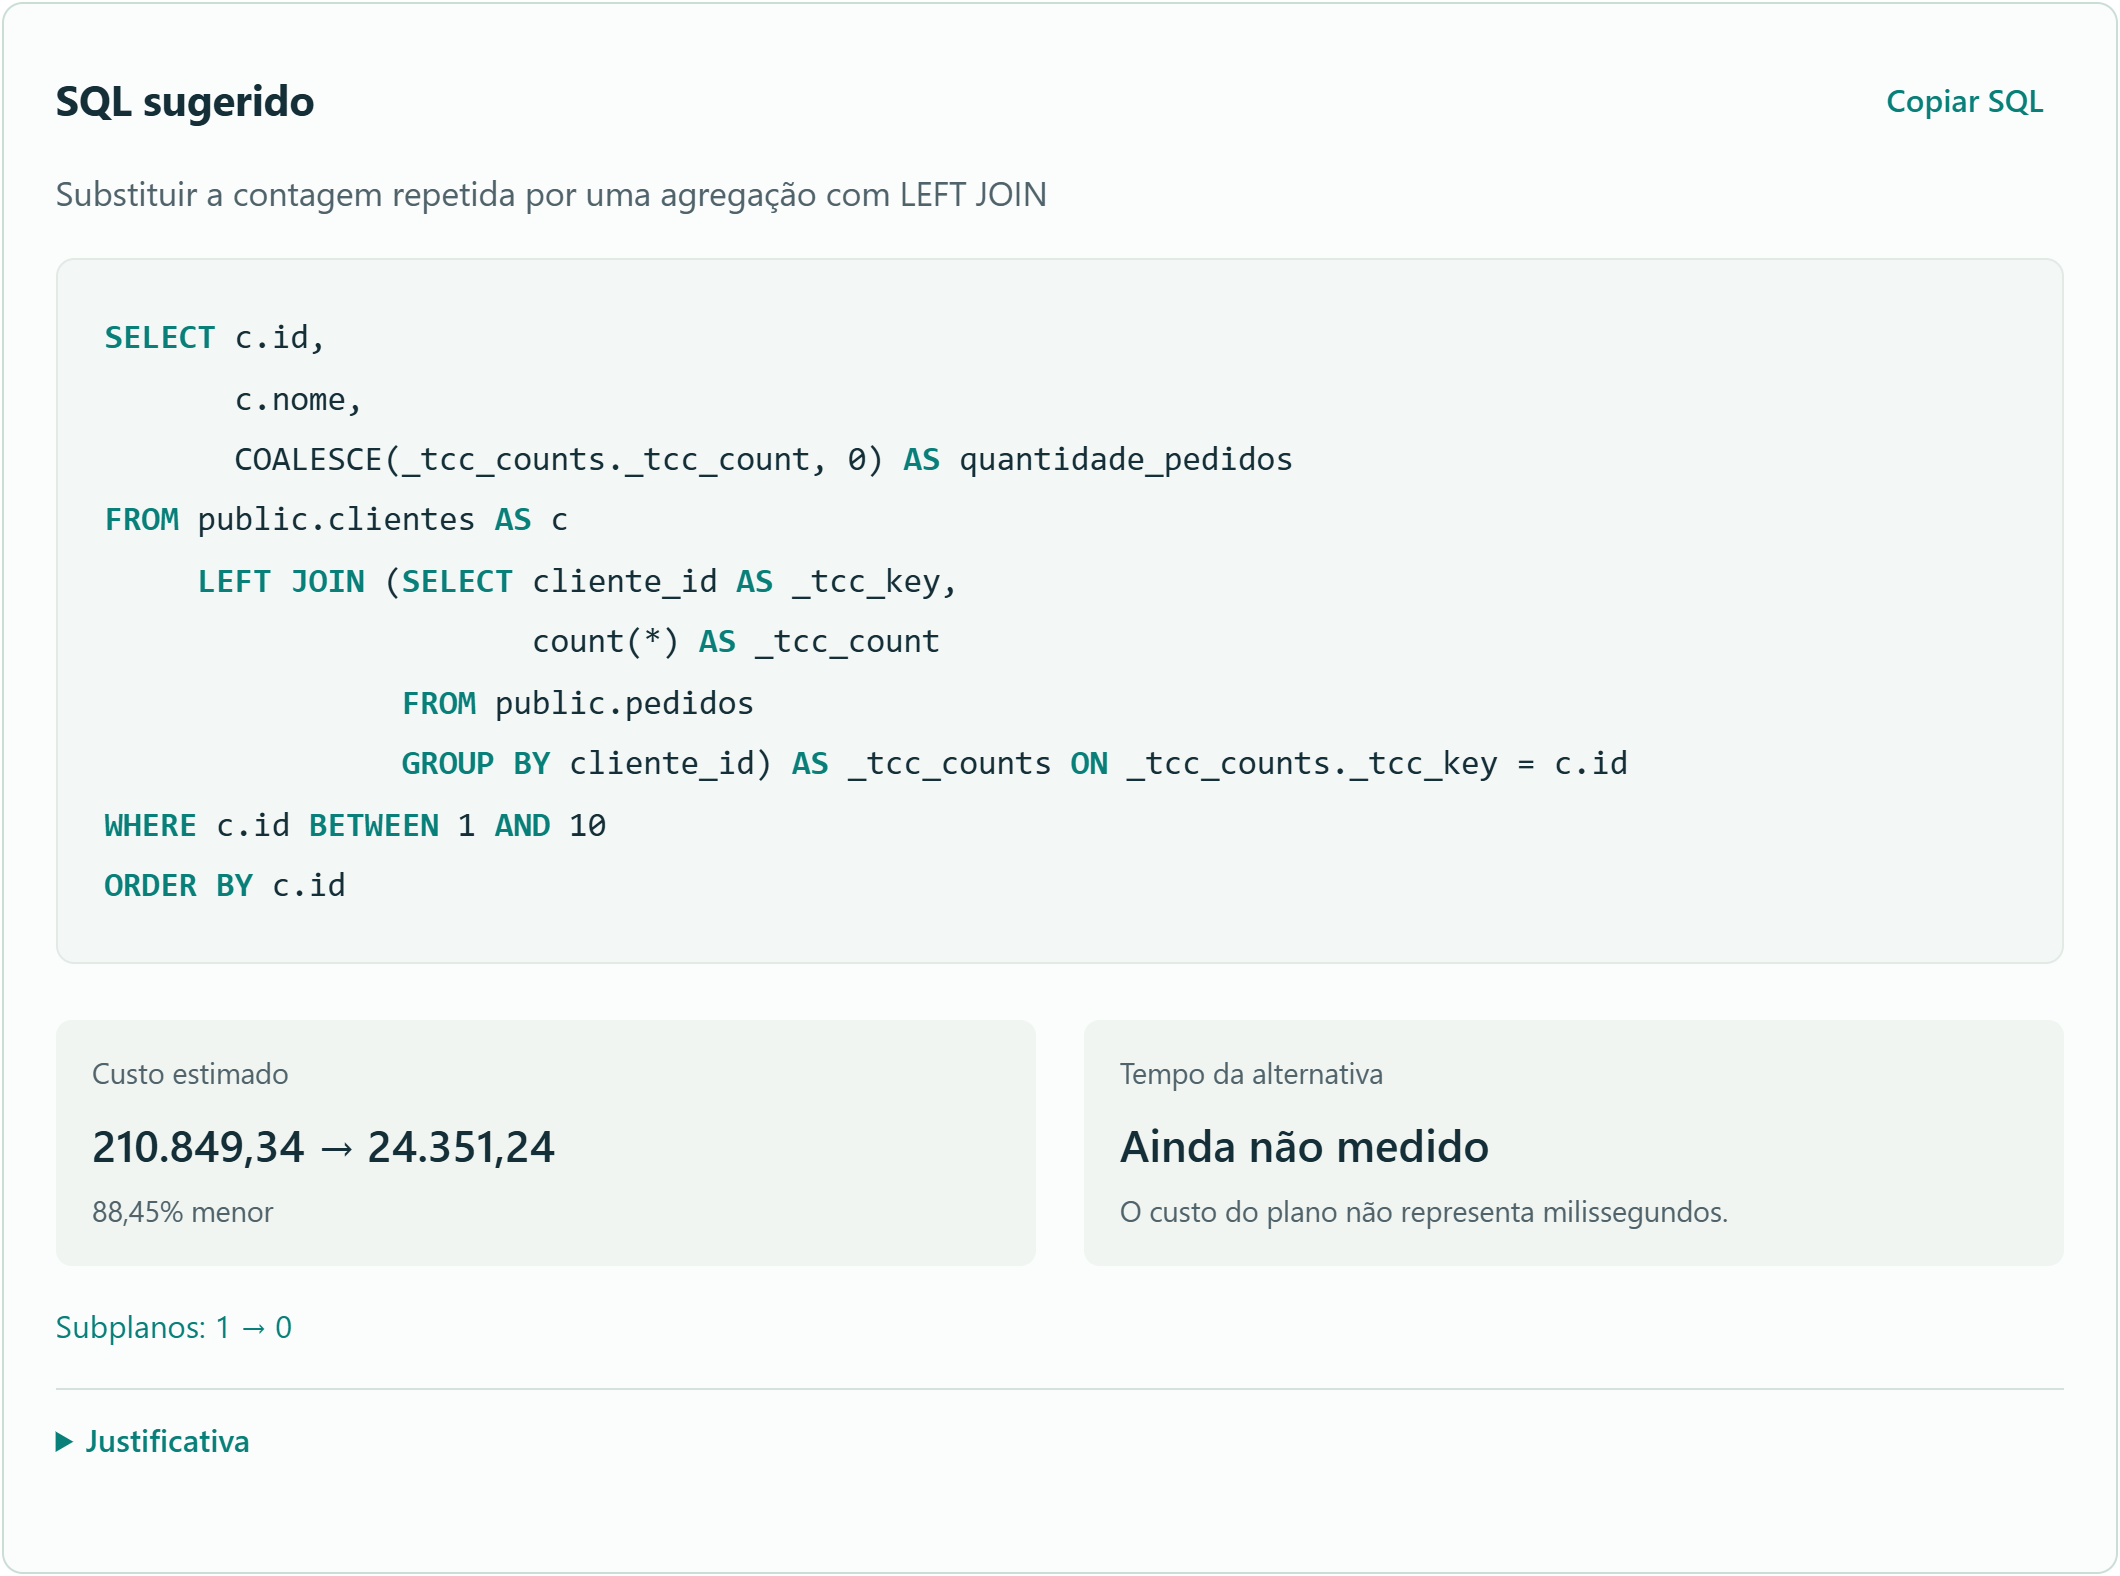
\includegraphics[width=\linewidth]{Figs/04_sugestao_otimizacao.png}
\par\smallskip
{\raggedright\footnotesize Fonte: do autor.\par}
\end{minipage}
\end{figure}



A Figura~\ref{fig:historico_medicao} apresenta uma avaliação experimental previamente concluída e armazenada no histórico do sistema. Para a consulta C03, foram realizadas 10 medições por versão, com tempos médios de 377,81 ms para a consulta original e 139,83 ms para a alternativa, representando uma redução de 62,99\%. Dessa forma, a interface permite acompanhar a investigação da consulta e consultar os resultados obtidos na avaliação experimental.


\begin{figure}[!htbp]
\centering
\caption{Resultado experimental da consulta C03 armazenado no histórico}
\label{fig:historico_medicao}
\begin{minipage}{0.95\textwidth}
\centering
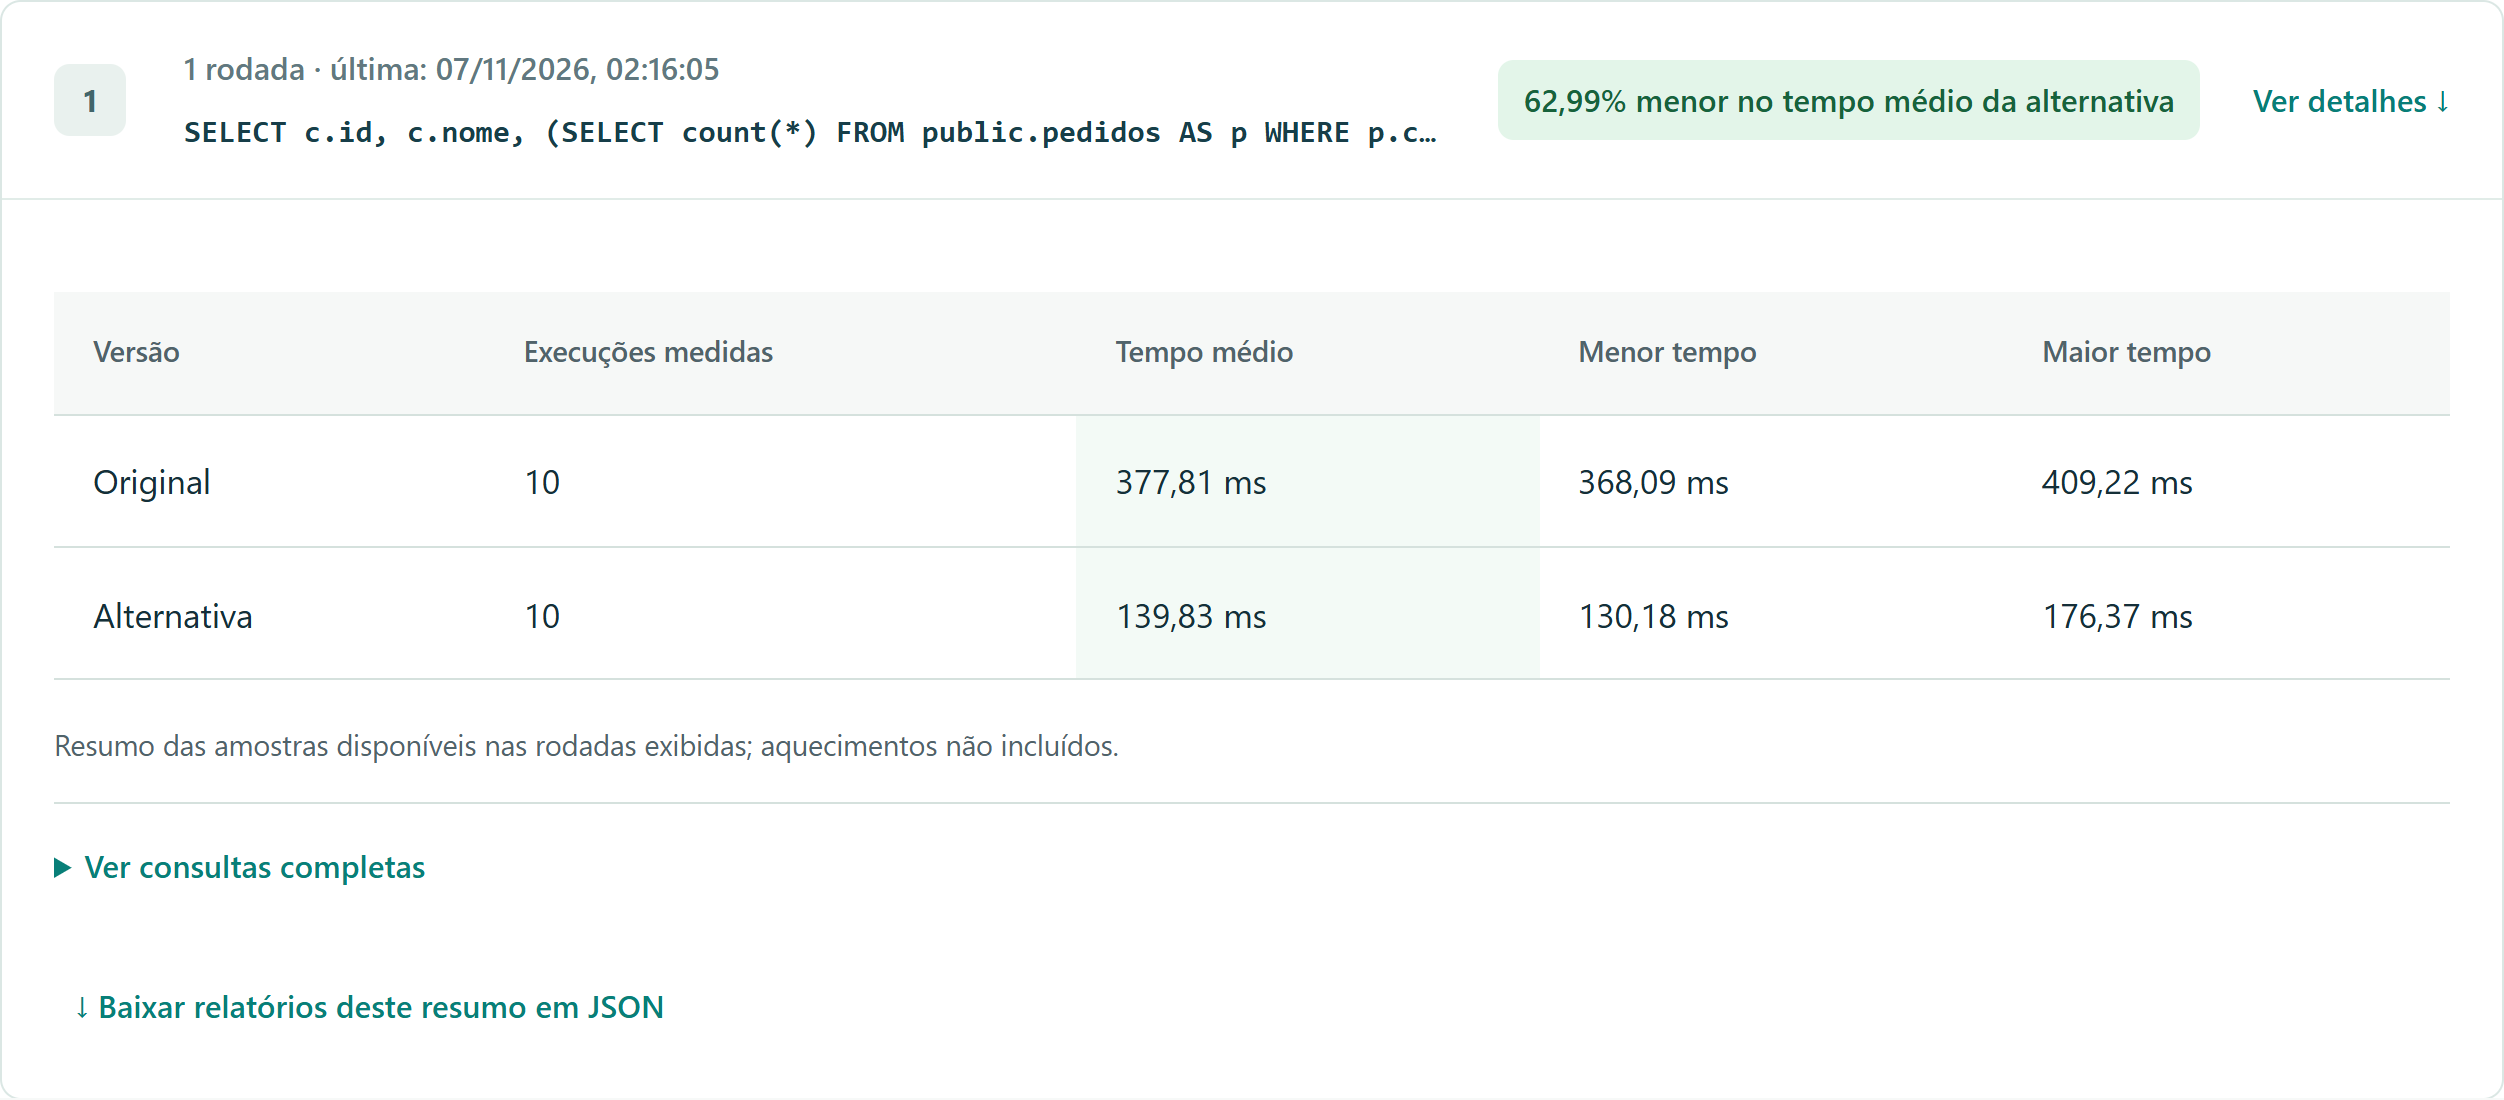
\includegraphics[width=\linewidth]{Figs/05_historico_medicao.png}
\par\smallskip
{\raggedright\footnotesize Fonte: do autor.\par}
\end{minipage}
\end{figure}

\FloatBarrier


\subsection{Discussão dos resultados experimentais}

Os resultados demonstraram que as alternativas de otimização apresentaram desempenhos diferentes conforme as características das consultas. Na busca por e-mail (C02), a remoção da função aplicada à coluna permitiu utilizar o índice existente, reduzindo o tempo médio em 99,89\%, considerando a normalização dos e-mails na base experimental. Também foram observadas reduções expressivas na contagem de pedidos por cliente (C03), de 62,99\%, e na contagem de pedidos por cliente e cidade (C12), de 88,29\%.

Por outro lado, as consultas C04 e C06 apresentaram aumentos de 4,15\% e 3,13\% no tempo médio, respectivamente. Esses resultados evidenciam que alterações na estrutura SQL não garantem melhorias de desempenho, reforçando a importância da validação experimental. Dessa forma, o protótipo demonstrou sua contribuição ao integrar a identificação de possíveis problemas, a apresentação de alternativas e a medição de seus efeitos.

\subsection{Limitações dos resultados}

A avaliação experimental utilizou dados fictícios e um ambiente controlado, com 12 consultas SQL e 10 medições por versão, realizadas em um único computador e sem simulação de usuários concorrentes. Os tempos podem variar conforme as condições de execução, e a correspondência dos resultados entre as consultas originais e alternativas foi verificada apenas para os dados e parâmetros utilizados. Portanto, os resultados obtidos não podem ser generalizados para todos os cenários.

O protótipo foi desenvolvido para PostgreSQL e utiliza estatísticas agregadas do \codigo{pg\_stat\_statements}, atualizadas mediante ação do usuário. Suas recomendações se limitam aos padrões SQL contemplados pelas regras implementadas, cujas pontuações não foram calibradas estatisticamente. Assim, a utilização em outros ambientes e cargas de trabalho requer avaliações adicionais.



%==========================================================================
% Conclusao
%==========================================================================

\section{CONCLUSÃO}

Este trabalho desenvolveu e avaliou um protótipo para auxiliar na identificação, análise e otimização de consultas SQL no PostgreSQL. A solução integrou a coleta de estatísticas de execução, a análise preventiva de planos, a identificação de possíveis problemas de desempenho e a apresentação de alternativas de otimização, permitindo avaliar seus efeitos por meio de medições experimentais.

A avaliação contemplou 12 consultas SQL, cada uma com uma alternativa de otimização, totalizando 240 execuções medidas. Os resultados demonstraram redução do tempo médio em 10 das 12 consultas. O maior ganho ocorreu na busca por e-mail, com redução de aproximadamente 99,89\%. Entretanto, duas alternativas apresentaram aumento no tempo médio, evidenciando que as modificações propostas nem sempre resultam em melhorias de desempenho.

Os resultados indicam que a integração entre estatísticas históricas, análise de planos e comparação experimental pode apoiar a investigação de consultas SQL e a avaliação de alternativas de otimização. O protótipo permitiu identificar possíveis problemas, apresentar recomendações e verificar os resultados das consultas antes das medições. Dessa forma, a solução atuou como ferramenta de apoio à decisão, sem realizar alterações automáticas no banco de dados.

Como trabalhos futuros, recomenda-se ampliar os experimentos para diferentes volumes de dados e condições de execução, incorporar novas regras de otimização e avaliar a solução em outros ambientes. Também podem ser realizados estudos com usuários para verificar a facilidade de utilização e a compreensão das recomendações apresentadas.


\section*{Declaração de Uso de Inteligência Artificial}
Os autores declaram que ferramentas de Inteligência Artificial generativa foram utilizadas exclusivamente como apoio auxiliar à elaboração deste trabalho, incluindo assistência na revisão linguística, estruturação textual e organização de ideias. Nenhuma ferramenta de IA foi utilizada para substituição da autoria intelectual, análise científica, interpretação dos resultados ou tomada de decisões acadêmicas. A responsabilidade integral pelo conteúdo, originalidade, veracidade das informações e conformidade com os princípios de integridade científica permanece integralmente atribuída aos autores.

%==========================================================================
% Referencias
%==========================================================================

\FloatBarrier


\bibliographystyle{abntex2-unesc}
\renewcommand{\refname}{REFERÊNCIAS}
\bibliography{referencias}


\end{document}

